%%%%%%%%%%%%%%%%%%%%%%%%%%%%%%%%%%%%%%%%%%%%%%%%%%%%%%%%%%%%%%%%%%%%%%
% How to use writeLaTeX: 
%
% You edit the source code here on the left, and the preview on the
% right shows you the result within a few seconds.
%
% Bookmark this page and share the URL with your co-authors. They can
% edit at the same time!
%
% You can upload figures, bibliographies, custom classes and
% styles using the files menu.
%
%%%%%%%%%%%%%%%%%%%%%%%%%%%%%%%%%%%%%%%%%%%%%%%%%%%%%%%%%%%%%%%%%%%%%%

\documentclass[12pt]{article}

\usepackage{sbc-template}

\usepackage{graphicx,url}

\usepackage[brazil]{babel}
\usepackage[utf8]{inputenc}

\usepackage{listings}
\usepackage{xcolor}

% Definição de cores personalizadas
\definecolor{mygreen}{rgb}{0,0.6,0}        % Para comentários
\definecolor{mygray}{rgb}{0.5,0.5,0.5}       % Para números de linha
\definecolor{mymauve}{rgb}{0.58,0,0.82}       % Para strings
\definecolor{myblue}{rgb}{0,0,0.8}            % Para palavras-chave
\definecolor{lightgray}{rgb}{0.95,0.95,0.95}  % Fundo dos códigos

% Configuração padrão para todos os códigos
\lstset{
  backgroundcolor=\color{lightgray},
  basicstyle=\ttfamily\footnotesize,
  breaklines=true,
  captionpos=b,
  numbers=left,
  numberstyle=\tiny\color{mygray},
  frame=single,
  keywordstyle=\color{myblue}\bfseries,
  commentstyle=\color{mygreen}\itshape,
  stringstyle=\color{mymauve},
  tabsize=4,
  showstringspaces=false,
  aboveskip=10pt,
  belowskip=5pt
}
% Estilo para código em C
\lstdefinestyle{CStyle}{
  language=C,
  % Outras opções específicas para C podem ser adicionadas aqui
}

% Definindo uma linguagem para CUDA baseada em C++
\lstdefinelanguage{CUDA}[]{C++}{
  morekeywords={__global__, __device__, __shared__, __host__},
  % Caso necessário, adicione mais palavras-chave ou opções específicas
}

% Estilo para código em CUDA
\lstdefinestyle{CUDAStyle}{
  language=CUDA,
  % Outras configurações específicas para CUDA podem ser adicionadas aqui
}

% Estilo para código em Python
\lstdefinestyle{PythonStyle}{
  language=Python,
  morekeywords=[2]{SequentialDiffusionEquation,with,OMPdiffusionEquation,CUDADiffusionEquation},
  % Outras opções específicas para Python podem ser adicionadas aqui
}

\renewcommand{\lstlistingname}{Código}

\sloppy

\title{Análise de Desempenho Paralelo de Modelos de Difusão de Contaminantes em
  Água}

\author{Eduardo Verissimo Faccio, Pedro Figueiredo Dias, \\
  Pedro Henrique de Oliveira Masteguin}

\address{Instituto de Ciência e Tecnologia -- Universidade Federal de São Paulo
  (UNIFESP)\\
  São José dos Campos -- SP -- Brasil
  \email{\{verissimo.eduardo,pedro.figueiredo,p.masteguin\}@unifesp.br}
}

\begin{document}

\maketitle

% \begin{resumo} 
%   Este meta-artigo descreve o estilo a ser usado na confecção de artigos e
%   resumos de artigos para publicação nos anais das conferências organizadas
%   pela SBC. É solicitada a escrita de resumo e abstract apenas para os artigos
%   escritos em português. Artigos em inglês deverão apresentar apenas abstract.
%   Nos dois casos, o autor deve tomar cuidado para que o resumo (e o abstract)
%   não ultrapassem 10 linhas cada, sendo que ambos devem estar na primeira
%   página do artigo.
% \end{resumo}

\section{Introdução}

A contaminação de corpos d'água, tais como lagos e rios, é um grande desafio ao
meio ambiente e a saúde pública, sendo preciso entender a dispersão do
contaminante no ambiente para poder realizar qualquer intervenção de mitigação.
Dessa forma, este trabalho foca na modelagem numérica da difusão de poluentes
em uma matriz bidimensional, utilizando o método de diferenças finitas para
aproximar a equação de difusão discreta:

\begin{equation}
  C_{i,j}^{t+1} = C_{i,j}^t + D \cdot \Delta t \cdot \left( \frac{C_{i+1,j}^t +
    C_{i-1,j}^t + C_{i,j+1}^t + C_{i,j-1}^t - 4 \cdot C_{i,j}^t}{\Delta x^2}
  \right)
  \label{eq:Difusao}
\end{equation}

Nesta equação, $C_{i,j}^t$ representa a concentração do contaminante na célula
$(i,j)$ no instante $t$, $D$ é o coeficiente de difusão, $\Delta t$ o intervalo
de tempo discreto e $\Delta x$ o espaçamento espacial. O objetivo principal é
desenvolver uma simulação que modele a difusão de contaminantes aplicando
programação paralela para acelerar os cálculos e analisar o comportamento dos
poluentes ao longo do tempo. Serão comparadas as versões sequencial e paralela
do algoritmo, utilizando OpenMP, CUDA e MPI para explorar o processamento
simultâneo em múltiplos núcleos e dispositivos. Os resultados serão validados
por meio de mapas de calor, gráficos de speedup e eficiência, além da
comparação das matrizes geradas. Este estudo demonstra como técnicas de
programação concorrente e distribuída podem otimizar simulações numéricas
complexas, reforçando os conceitos aprendidos na disciplina e demonstrando sua
aplicação prática no desenvolvimento de soluções eficientes.

\section{Implementação do Algorítimo}

\subsection{Código Sequencial}

O código sequencial implementa a solução numérica da equação de difusão usando
uma abordagem serial. Utilizando-se do método de diferenças finitas, é simulado
a dispersão de uma substância em uma matriz bidimensional. Cada célula da
matriz representa a concentração de uma substância em um ponto do espaço.

O cálculo é realizado em um laço de repetição que itera sobre todas as células
da matriz. A atualização de cada célula depende da média das concentrações dos
seus vizinhos imediatos e de parâmetros físicos como coeficiente de difusão, o
intervalo de tempo $\Delta t$ e o espaçamento espacial $\Delta x$.

\begin{lstlisting}[style=CStyle, caption={Código sequencial da para cálculo da difusão, que será utilizado como base para as demais implementações.}, label={cod:seq}]
double sequential_diff_eq(double **C, double **C_new, DiffEqArgs *args) {
    int N = args->N;
    double D = args->D;
    double DELTA_T = args->DELTA_T;
    double DELTA_X = args->DELTA_X;
    double difmedio = 0.;

    for (int i = 1; i < N - 1; i++) {
        for (int j = 1; j < N - 1; j++) {
            C_new[i][j] = C[i][j] + D * DELTA_T * ((C[i + 1][j] + C[i - 1][j] + C[i][j + 1] + C[i][j - 1] - 4 * C[i][j]) / (DELTA_X * DELTA_X));
            difmedio += fabs(C_new[i][j] - C[i][j]);
        }
    }

    return difmedio / ((N - 2) * (N - 2));
}
\end{lstlisting}

\subsection{Código Paralelo em Open Multi-Processing (OMP)}

A implementação paralela utiliza a biblioteca OpenMP para distribuir a carga de
trabalho entre múltiplos núcleos, mantendo a lógica do algoritmo sequencial.
Essa distribuição é realizada através de diretivas específicas inseridas na
estrutura do código original.

\begin{lstlisting}[style=CStyle, caption={Implementação paralelizada utilizando a biblioteca OpenMP.}, label={cod:omp}]
double omp_diff_eq(double **C, double **C_new, DiffEqArgs *args) {
    int N = args->N;
    double D = args->D;
    double DELTA_T = args->DELTA_T;
    double DELTA_X = args->DELTA_X;
    double difmedio = 0.;

#pragma omp parallel for collapse(2) reduction(+ : difmedio)
    for (int i = 1; i < N - 1; i++) {
        for (int j = 1; j < N - 1; j++) {
            C_new[i][j] = C[i][j] + D * DELTA_T * ((C[i + 1][j] + C[i - 1][j] + C[i][j + 1] + C[i][j - 1] - 4 * C[i][j]) / (DELTA_X * DELTA_X));
            difmedio += fabs(C_new[i][j] - C[i][j]);
        }
    }

    return difmedio / ((N - 2) * (N - 2));
}
\end{lstlisting}

\begin{description}
  \item[\texttt{\#pragma omp parallel for collapse(2)}:]
        Esta diretiva divide automaticamente os laços de cálculo entre diversos \textit{threads}. Cada \textit{thread} é responsável por atualizar uma parte distinta da matriz, permitindo que várias seções do cálculo sejam processadas simultaneamente. O parâmetro \texttt{collapse(2)} indica que os dois laços aninhados serão combinados para otimizar o paralelismo.

  \item[\texttt{\#pragma omp parallel for reduction(+:difmedio) collapse(2)}:]
        Assim como a diretiva anterior, esta instrução paraleliza as iterações do laço, porém com o acréscimo de uma operação de redução. Essa redução garante que o somatório, utilizado para monitorar a convergência do algoritmo, seja realizado de forma segura entre os diferentes \textit{threads}.

  \item[\texttt{omp\_set\_num\_threads(int num\_threads)}:]
        Esta função permite configurar dinamicamente o número de \textit{threads} a serem utilizados, sendo essencial para testes e análises de desempenho.
\end{description}

\subsection{Código Paralelo em CUDA}

Nesta implementação, o algoritmo de difusão foi otimizado para execução em
GPUs, aproveitando a arquitetura CUDA (Compute Unified Device Architecture). A
abordagem distribui o cálculo da atualização das células da matriz de
concentração entre milhares de \texttt{threads}, onde cada uma processa
individualmente uma célula da matriz utilizando o método de diferenças finitas.
Essa estratégia maximiza a paralelização, resultando em desempenho superior
quando comparada às implementações sequencial e mesmo às paralelas em CPU.

\begin{lstlisting}[style=CUDAStyle, caption={Implementação paralelizada utilizando CUDA.}, label={cod:cuda}]
__global__ void diffusion_kernel(double *C, double *C_new, double *block_sums, int N, double D, double DELTA_T, double DELTA_X) {
    extern __shared__ double sdata[]; 

    int i = blockIdx.y * blockDim.y + threadIdx.y + 1;
    int j = blockIdx.x * blockDim.x + threadIdx.x + 1;

    double diff_val = 0.0f;

    if (i < N - 1 && j < N - 1) {
        int idx = i * N + j;
        double up = C[(i - 1) * N + j];
        double down = C[(i + 1) * N + j];
        double left = C[i * N + (j - 1)];
        double right = C[i * N + (j + 1)];
        double center = C[idx];

        C_new[idx] = center + D * DELTA_T * ((up + down + left + right - 4 * center) / (DELTA_X * DELTA_X));

        diff_val = fabs(C_new[idx] - center);
    }

    int tid = threadIdx.y * blockDim.x + threadIdx.x;
    sdata[tid] = diff_val;
    __syncthreads();

    for (unsigned int s = (blockDim.x * blockDim.y) / 2; s > 32; s >>= 1) {
        if (tid < s) {
            sdata[tid] += sdata[tid + s];
        }
        __syncthreads();
    }

    if (tid < 32) {
        volatile double *vsmem = sdata;
        vsmem[tid] += vsmem[tid + 32];
        vsmem[tid] += vsmem[tid + 16];
        vsmem[tid] += vsmem[tid + 8];
        vsmem[tid] += vsmem[tid + 4];
        vsmem[tid] += vsmem[tid + 2];
        vsmem[tid] += vsmem[tid + 1];
    }

    if (tid == 0) {
        block_sums[blockIdx.y * gridDim.x + blockIdx.x] = sdata[0];
    }
}
\end{lstlisting}

O kernel \texttt{diffusion\_kernel} é responsável por calcular a nova
concentração de cada célula com base nos valores dos seus vizinhos imediatos,
aplicando a fórmula de difusão que incorpora os parâmetros de difusão, tempo e
espaço. Este kernel é lançado em uma grade (\textit{grid}) composta por blocos
de \texttt{threads}, cujas dimensões podem ser configuradas dinamicamente
através da função \texttt{set\_block\_dimensions}. A utilização de memória
compartilhada (\texttt{\_\_shared\_\_}) acelera a acumulação dos valores
diferenciais, facilitando a verificação da convergência do algoritmo.

\textbf{Etapas do Fluxo de Execução:}
\begin{enumerate}
  \item \textbf{Inicialização (\texttt{cuda\_init}):}
        Aloca a memória necessária na GPU e transfere os dados iniciais da CPU para a memória do dispositivo.
  \item \textbf{Execução do Kernel (\texttt{cuda\_diff\_eq}):}
        Lança o kernel que atualiza os valores da matriz e calcula a diferença média entre iterações.
  \item \textbf{Recuperação dos Dados (\texttt{cuda\_get\_result}):}
        Transfere os resultados computados na GPU de volta para a CPU.
  \item \textbf{Finalização (\texttt{cuda\_finalize}):}
        Libera a memória previamente alocada na GPU.
\end{enumerate}

Para facilitar a implementação do algoritmo \textit{stencil} na GPU, a matriz
bidimensional foi convertida em um vetor unidimensional, onde as linhas são
concatenadas. Essa abordagem simplifica o acesso à memória, exigindo apenas um
cálculo cuidadoso dos índices para que cada \textit{thread} acesse o elemento
correto.

Para a operação de redução, cada \textit{thread} inicialmente armazena sua
contribuição em memória compartilhada. Em seguida, o kernel realiza uma soma
hierárquica, agregando os valores de forma progressiva até que reste um único
valor por bloco. Esse resultado final é copiado para a memória global,
possibilitando o cálculo da diferença média total já na CPU e,
consequentemente, a verificação da convergência do algoritmo.

Adicionalmente, a função \texttt{set\_block\_dimensions} possibilita o ajuste
das dimensões dos blocos de \textit{threads}, permitindo a experimentação com
diferentes granularidades de paralelismo para um balanceamento eficiente da
carga entre os multiprocessadores da GPU.

\subsection{Interface Python e ferramenta CMake}

O projeto utiliza o CMake como sistema de compilação para gerenciar processos e
dependências tanto da implementação em OpenMP quanto da versão CUDA, definindo
tudo por meio de arquivos de configuração. Para destacar as diferenças de
desempenho entre as abordagens sequencial, OpenMP e CUDA, as otimizações do
compilador — como a vetorização automática que inicialmente minimizava essas
disparidades — são desabilitadas por meio de flags específicas, permitindo uma
execução mais direta e comparável.

Paralelamente, foi implementada uma interface Python usando o módulo
\textit{ctypes} para carregar dinamicamente as bibliotecas compiladas e mapear
suas funções, facilitando a integração com métodos de análise e visualização
desenvolvidos em notebooks Jupyter. Inspirada em bibliotecas como o NumPy, essa
abordagem combina a eficiência das implementações em C com a flexibilidade e a
facilidade de uso do Python, possibilitando a configuração de parâmetros como
tamanho da matriz, coeficiente de difusão e dimensões dos blocos de
\textit{threads}.

\begin{lstlisting}[style=PythonStyle, caption={Implementação paralelizada utilizando CUDA.}, label={cod:pythonlib}]
from diffusion import (
    SequentialDiffusionEquation,
    OMPdiffusionEquation,
    CUDADiffusionEquation,
)

lib_path = "./build/libDiffusionEquation.so"

# Context manager is not necessary for sequential and OMP
# solver, but it is recommended to use it even for them
with SequentialDiffusionEquation(
    library_path=lib_path, N=200, D=0.05, DELTA_T=0.02, DELTA_X=1.0,
    initial_concentration_points={(100, 100): 1.0},
) as seq_solver:

    for _ in range(1000): # Perform 1000 simulation steps
        diff_seq = seq_solver.step()  # Execute the C code step
    
    value_at_center = seq_solver.concentration_matrix[100][100]
    print(f"Sequential diffusion value at center: {value_at_center}")


with OMPdiffusionEquation(
    library_path=lib_path, N=200, D=0.05, DELTA_T=0.02, DELTA_X=1.0,
    initial_concentration_points={(100, 100): 1.0},
) as omp_solver:

    for _ in range(1000):
        diff_omp = omp_solver.step()  # Execute the OpenMP step
    
    value_at_center = omp_solver.concentration_matrix[100][100]
    print(f"OMP diffusion value at center: {value_at_center}")


# Context manager is necessary for CUDA solver
# You also can free them manually by calling the finalize method
with CUDADiffusionEquation(
    library_path=lib_path, N=200, D=0.05, DELTA_T=0.02, DELTA_X=1.0,
    initial_concentration_points={(100, 100): 1.0},
) as cuda_solver:

    for _ in range(1000):
        diff_cuda = cuda_solver.step()  # Execute the cuda step
    
    cuda_solver.get_result() # Get the result from the device to the host
    value_at_center = cuda_solver.concentration_matrix[100][100]
    print(f"CUDA diffusion value at center: {value_at_center}")
\end{lstlisting}

\section{Resultados}

Nesta seção, apresentamos os resultados obtidos de nossa implementação.
Inicialmente, analisamos a equivalência lógica entre os códigos sequencial e
paralelo, considerando possíveis erros que podem surgir na paralelização, como
condições de corrida ou inconsistências de sincronização. Em seguida,
ilustramos, por meio de mapas de calor, a atualização dos valores da matriz ao
longo do tempo. Por fim, realizamos uma análise comparativa dos tempos médios
de execução e \textit{speedup} entre as duas versões.

\subsection{Validação da Implementação - Numérico}

Para assegurar a correção das duas implementações, verificamos em cada iteração
se os valores presentes em cada célula da matriz são idênticos. Dessa forma, o
resultado na última iteração deve ser o mesmo em ambas as versões.

Por meio desse procedimento, utilizando a interface Python em conjunto com um
Jupyter Notebook, comprovamos que as duas soluções produzem resultados
idênticos. Isso era esperado, pois no código paralelo não ocorrem condições de
corrida, uma vez que a escrita não é realizada na mesma região de memória das
leituras, tornando o processamento de cada célula pelas \textit{threads}
independente.

\subsection{Validação da Implementação - Ilustrativo}

Para ilustrar o funcionamento da implementação, foram gerados mapas de calor,
representado pela Figura~\ref{fig:heatmap}, nos quais cada ponto de uma matriz
50$\times$50 é representado por uma cor distinta. Cores escuras correspondem a
valores próximos de um, indicando alta concentração do contaminante, enquanto
cores claras representam valores próximos de zero, indicando baixa presença de
contaminação.

\begin{figure}[ht]
  \centering
  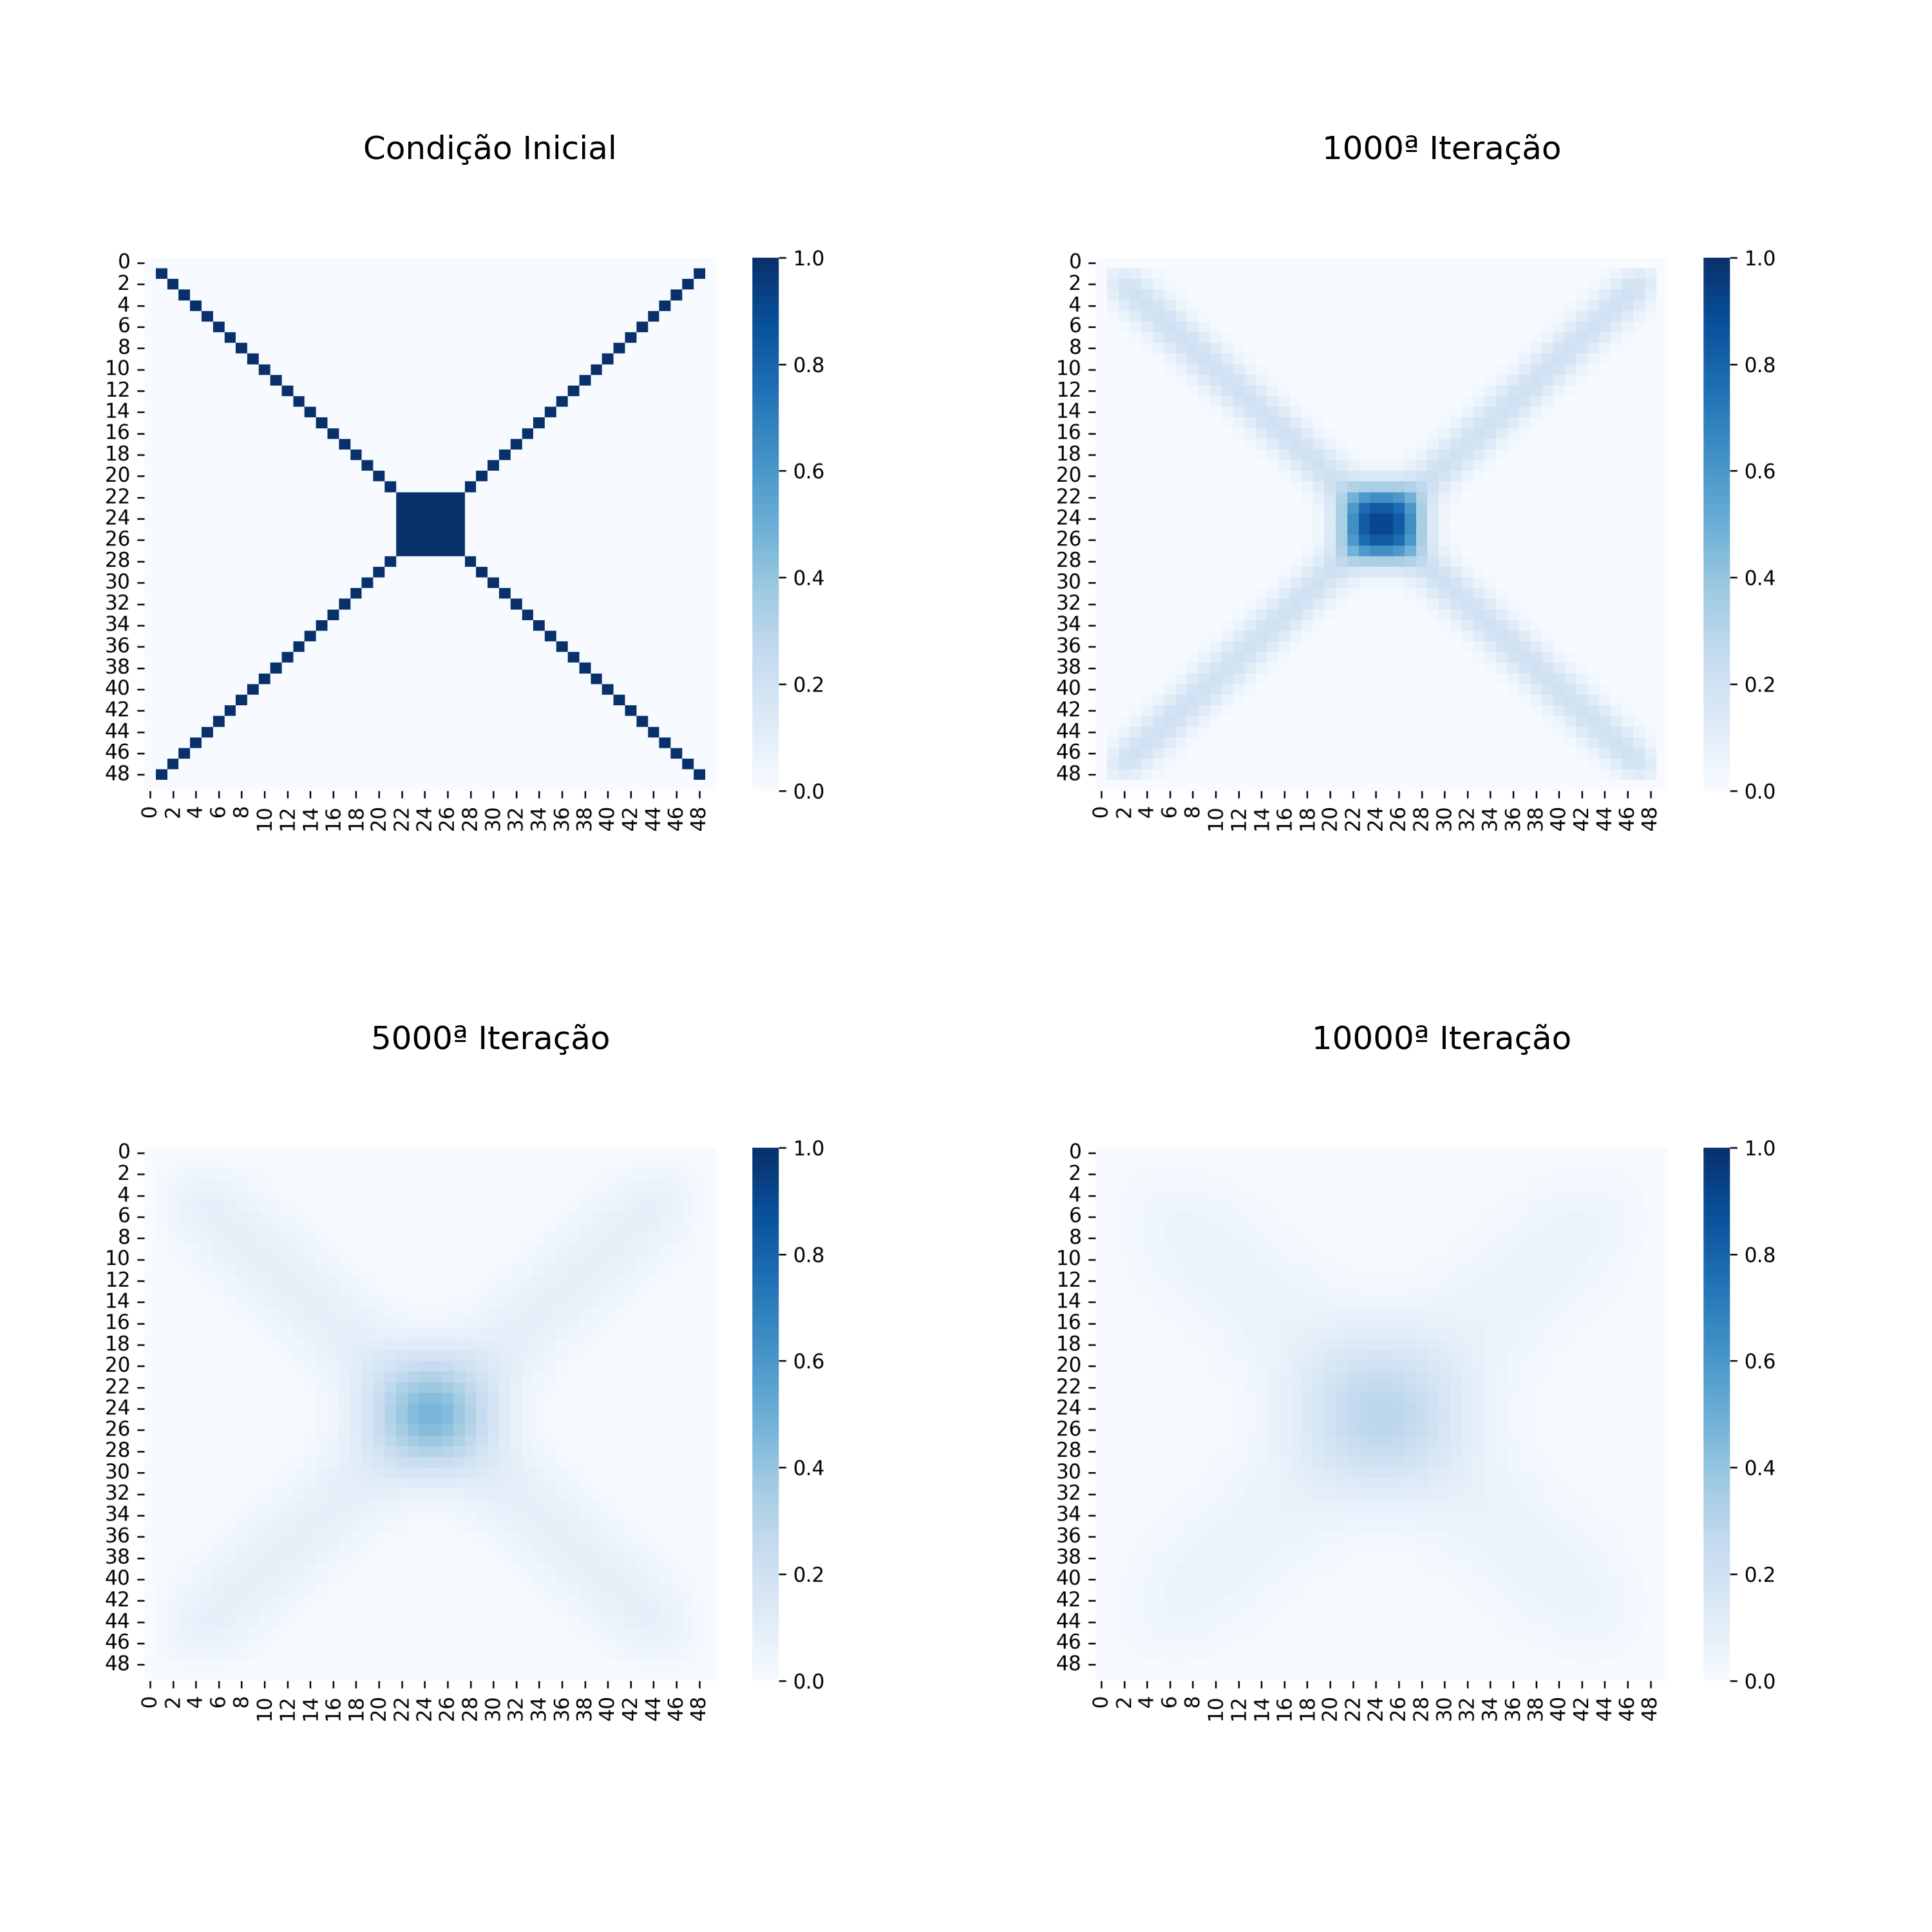
\includegraphics[width=.5\textwidth]{figs/heatmap.png}
  \caption{Mapa de calor em quatro instantes distintos da simulação.}\label{fig:heatmap}
\end{figure}

Analisando a progressão dos mapas de calor, observamos que o comportamento faz
sentido no contexto da solução proposta. Inicialmente, o contaminante é
adicionado com alta concentração nas diagonais e no centro da matriz,
evidenciado pelas regiões azuis-escuros. Com o avanço das iterações, o
contaminante começa a se difundir para as regiões adjacentes, aumentando
gradativamente a luminosidade nessas áreas e diminuindo nos pontos de
concentração inicial. Na última iteração, a concentração se distribui
uniformemente pela matriz, com valores próximos entre si.

\subsection{Análise de Desempenho}

A análise de desempenho foi realizada em um computador \textit{desktop} com as
especificações apresentadas na Tabela~\ref{tab:especificacaoHardware}. Ademais,
as especificações dos parâmetros do problema foram incluídas na
Tabela~\ref{tab:especificacaoSimulacao}.

\begin{table}[ht]
  \centering
  \caption{Tabela de especificação de Hardware}
  \vspace{0.3cm}
  \begin{tabular}{||c c||}
    \hline
    Especificações      & Detalhes                         \\ [0.5ex]
    \hline\hline
    Processador         & Intel i7--7500U @ 2.7GHz--3.5GHz \\
    \hline
    Núcleos / Lógicos   & 2 / 4                            \\
    \hline
    Memória RAM         & 10 GB                            \\
    \hline
    Sistema Operacional & Ubuntu 22.04.05 (via WSL)        \\
    \hline
    GPU                 & NVIDIA GeForce 940MX - 2GB VRAM  \\
    \hline
  \end{tabular}\label{tab:especificacaoHardware}
\end{table}

\begin{table}[ht]
  \centering
  \caption{Tabela de especificação da Simulação}
  \vspace{0.3cm}
  \begin{tabular}{||c c||}
    \hline
    Especificações                    & Detalhes                    \\ [0.5ex]
    \hline\hline
    Dimensão da Matriz (N $\times$ N) & 3000 $\times$ 3000          \\
    \hline
    Número de Iterações               & 1000                        \\
    \hline
    Distribuição Inicial              & Alta concentração no centro \\
    \hline
    Coeficiente de Difusão            & 0.1                         \\
    \hline
    $\Delta t$                        & 0.01                        \\
    \hline
    $\Delta x$                        & 1.0                         \\
    \hline
  \end{tabular}\label{tab:especificacaoSimulacao}
\end{table}

Para obter valores mais consistentes e minimizar influências externas, como
outros programas em execução, cada teste foi executado quinze vezes e, assim,
calculamos o tempo médio gasto e seu desvio padrão. O \textit{speedup} é
calculado dividindo-se o tempo de execução sequencial pelo tempo de execução
CUDA correspondente.

\begin{table}[ht]
  \centering
  \caption{Tabela de comparação de desempenho entre o código sequencial e o
    utilizando CUDA.}\label{tab:Resultados}
  \vspace{0.3cm}
  \begin{tabular}{||c c c||}
    \hline
    Experimento   & Tempo            & SpeedUp \\ [0.5ex]
    \hline\hline
    Sequencial    & 27.23 $\pm$ 2.36 & 1.0     \\
    \hline
    OMP (1T)      & 26.33 $\pm$ 1.09 & 1.03    \\
    \hline
    OMP (2T)      & 16.58 $\pm$ 1.72 & 1.64    \\
    \hline
    OMP (4T)      & 13.34 $\pm$ 1.52 & 2.04    \\
    \hline
    OMP (8T)      & 13.38 $\pm$ 1.54 & 2.35    \\
    \hline
    OMP (16T)     & 13.75 $\pm$ 1.42 & 1.98    \\
    \hline
    OMP (32T)     & 13.96 $\pm$ 1.46 & 1.95    \\
    \hline
    MPI (1P)      & 25.47 $\pm$ 1.64 & 1.07    \\
    \hline
    MPI (2P)      & 16.51 $\pm$ 1.61 & 1.65    \\
    \hline
    MPI (4P)      & 13.53 $\pm$ 1.52 & 2.01    \\
    \hline
    MPI (8P)      & 15.88 $\pm$ 1.71 & 1.71    \\
    \hline
    MPI (16P)     & 18.03 $\pm$ 1.40 & 1.51    \\
    \hline
    MPI (32P)     & 19.60 $\pm$ 1.51 & 1.39    \\
    \hline
    CUDA (16, 16) & 5.23 $\pm$ 1.04  & 5.21    \\
    \hline
  \end{tabular}
\end{table}

\begin{figure}[ht]
  \centering
  \begin{minipage}[b]{0.37\textwidth}
    \centering
    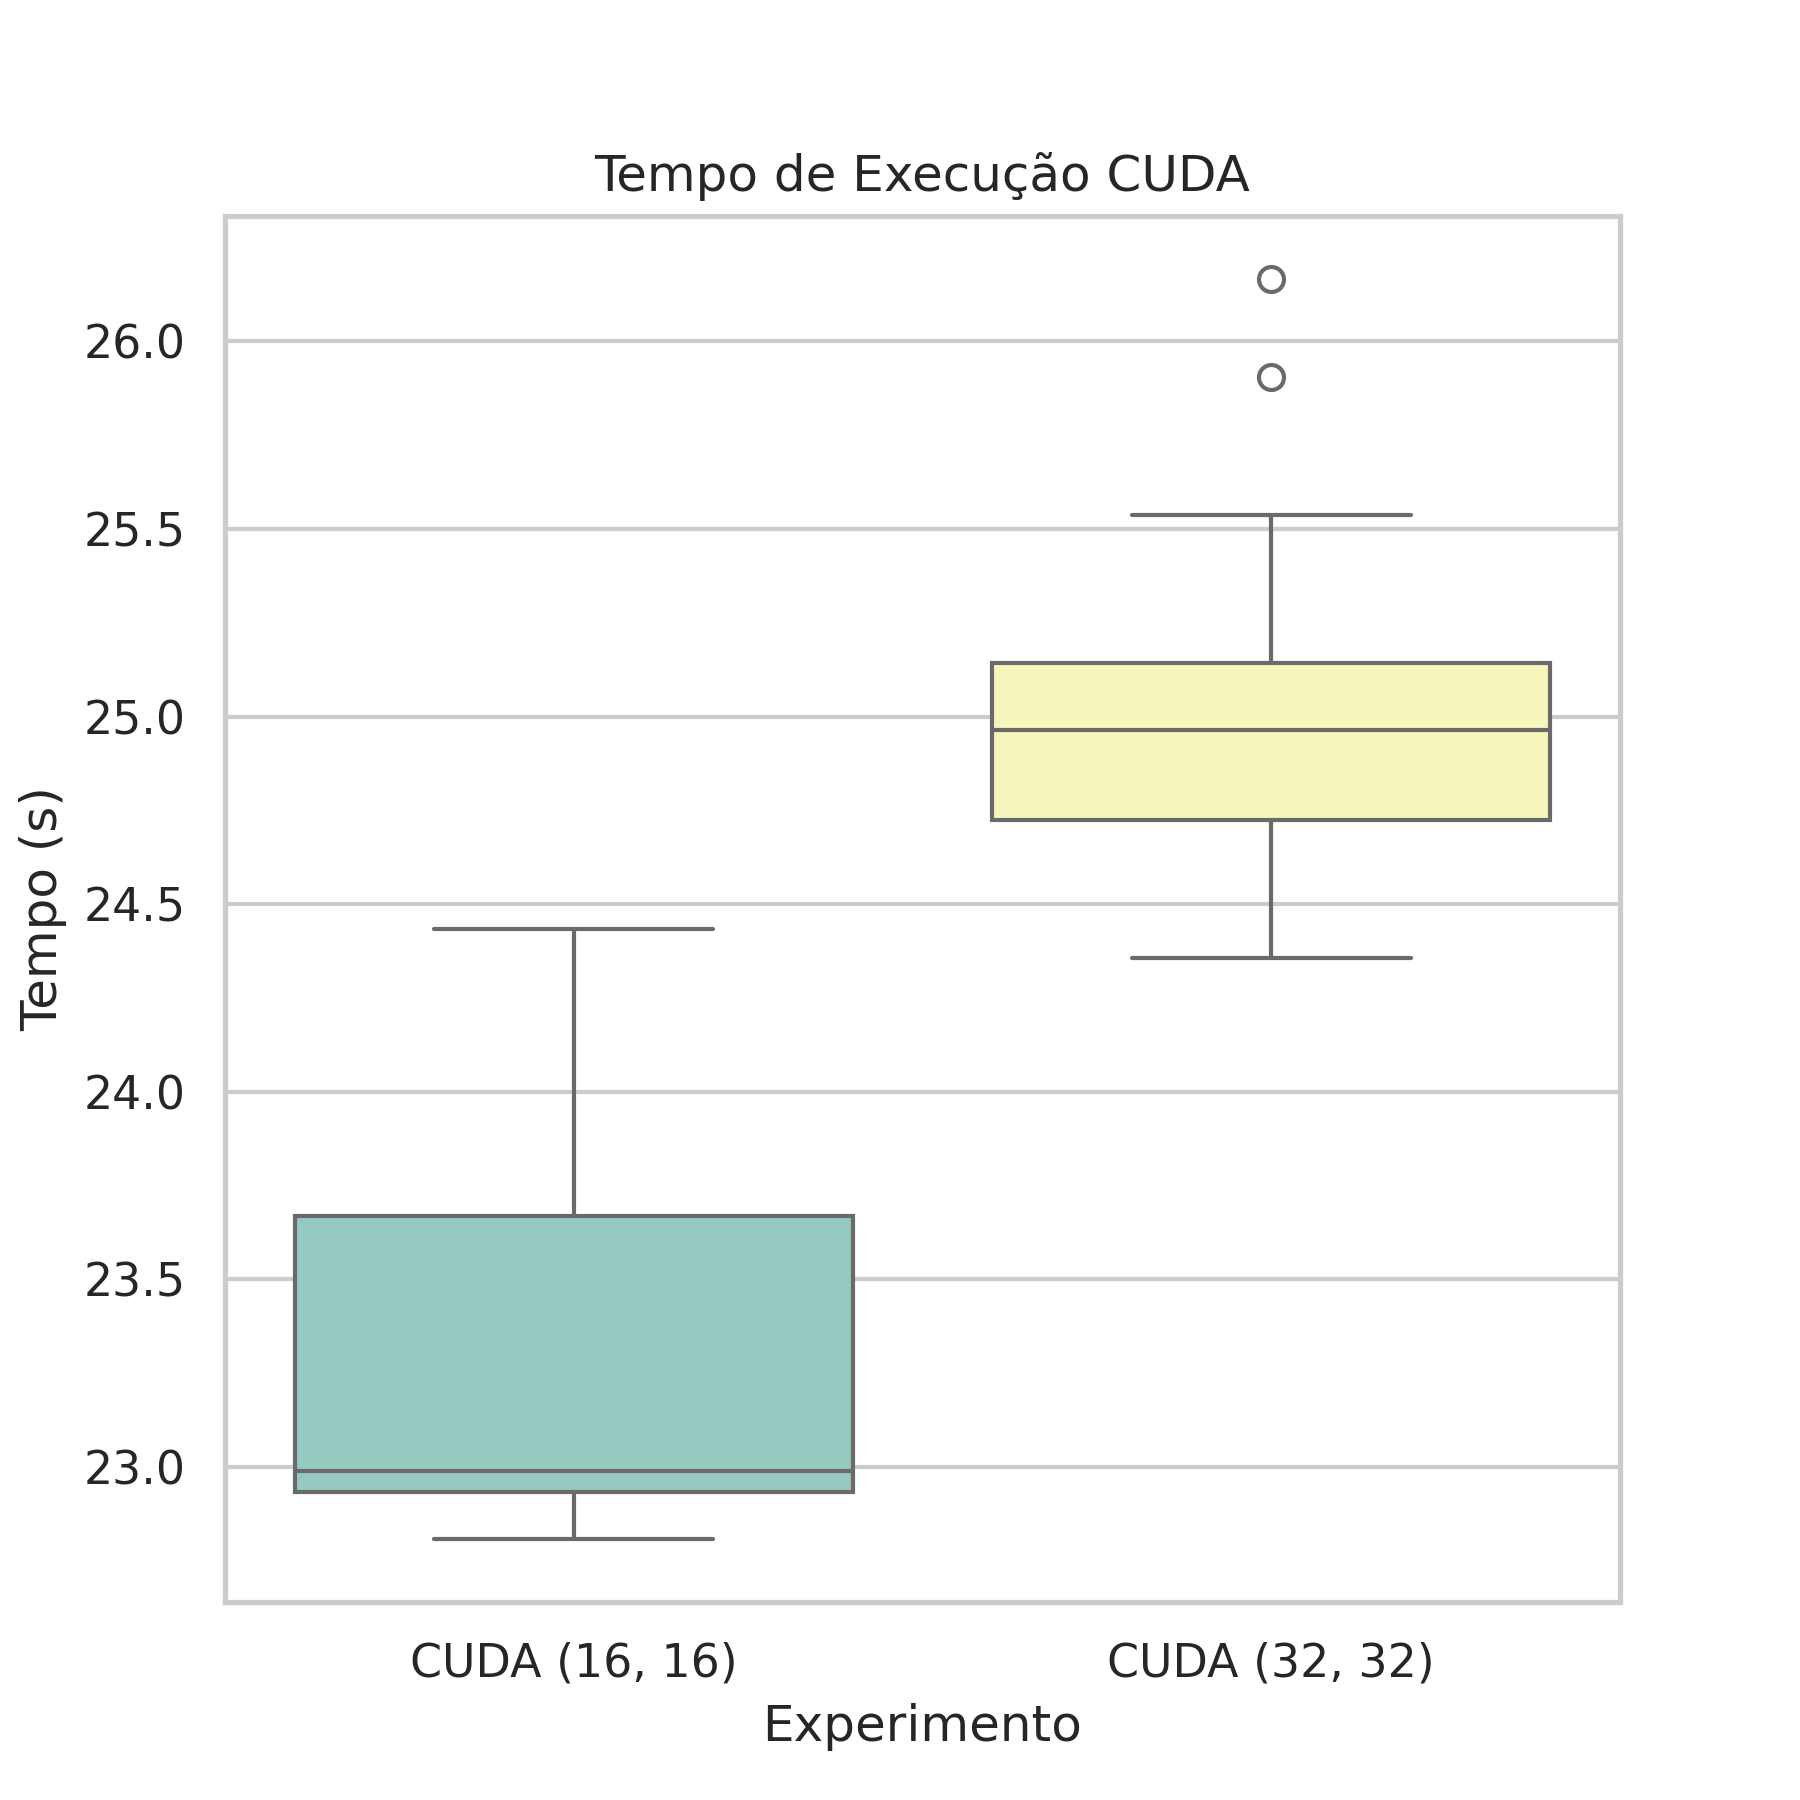
\includegraphics[width=\textwidth]{figs/times_boxplot_cuda.png}
  \end{minipage}
  \begin{minipage}[b]{0.25\textwidth}
    \centering
    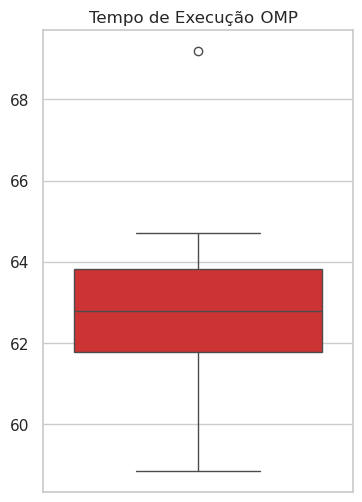
\includegraphics[width=\textwidth]{figs/times_boxplot_omp.png}
  \end{minipage}
  \begin{minipage}[b]{0.25\textwidth}
    \centering
    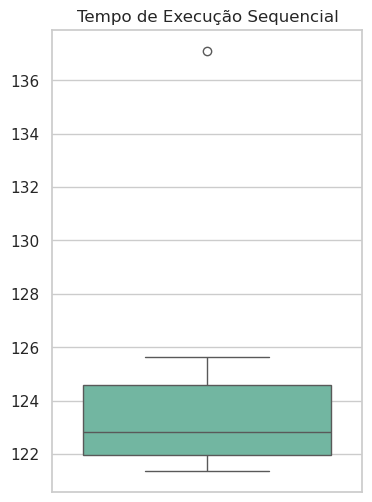
\includegraphics[width=\textwidth]{figs/times_boxplot_sequential.png}
  \end{minipage}
  \caption{Gráficos \textit{boxplots} para os tempos de execução medidos para cada um dos experimentos registrados na Tabela~\ref{tab:Resultados}. }\label{fig:Boxplots}
\end{figure}

A visualização dos dados por meio de gráficos de \textit{boxplot}
(Figura~\ref{fig:Boxplots}) é um ótimo meio para avaliar o desempenho do
algoritmo, considerando as possíveis incertezas que advêm do sistema
computacional em que ele está inserido. Problemas de priorização de tarefas,
alocação de recursos e utilização do sistema pelo usuário podem introduzir
variações significativas no tempo de execução e na eficiência geral do
algoritmo. Essas flutuações são facilmente identificadas por meio dos gráficos,
ilustrando que existe uma pequena diferença de poucos segundos que podem
influenciar no tempo de execução final do programa.

Nota-se uma grande eficiência do tempo de execução do algoritmo de CUDA em
relação ao sequencial e OpenMP, o que demonstra o quão importante esse hardware
pode ser para tarefas que demandam cálculos extremos, como os de aprendizado de
máquina, por exemplo. Porém, importante ressaltar que esse ganho será menor se
o tamanho da simulação for reduzido, já que todo o processo de alocar, enviar e
receber dados e administrar a GPU possui um custo, que pode ser evitado ao
utilizar apenas as threads da própria CPU\@.

O desempenho inferior do CUDA com \textit{block dim} (32, 32) em relação ao
(16, 16) ocorre porque blocos maiores podem causar um maior uso de recursos,
como memória compartilhada e registradores, levando à saturação da capacidade
da GPU\@. Isso resulta em maior latência devido à competição entre blocos por
recursos limitados.

\section{Conclusão}

Com a introdução da implementação paralela utilizando CUDA, além da sequência e
da versão OpenMP previamente analisadas, validou-se a correção dos resultados
ao longo das diferentes abordagens e examinou-se o impacto do paralelismo no
tempo de execução. Os experimentos demonstraram que, embora a paralelização com
CUDA proporcione ganhos significativos em relação ao código sequencial, podem
existir limitações na escalabilidade, que são decorrentes de \textit{overheads}
de comunicação entre a CPU e a GPU, latências de memória e restrições
arquiteturais do próprio hardware gráfico.

Dessa forma, o estudo evidencia não apenas as vantagens práticas da
paralelização em termos de desempenho e eficiência em simulações numéricas, mas
também ressalta a importância de se compreender os desafios inerentes às
diferentes estratégias paralelas. A experiência com CUDA complementa os
conceitos fundamentais aprendidos em programação concorrente e distribuída,
oferecendo percepções valiosas sobre a aplicabilidade e os limites da
aceleração por GPU em contextos computacionais exigentes.

\bibliographystyle{sbc}
\bibliography{sbc-template}
\nocite{*}
\end{document}